\documentclass[11pt]{report}
\usepackage[french]{babel}
\usepackage[utf8]{inputenc}
\usepackage[T1]{fontenc}
\usepackage[top = 2cm, bottom = 2cm, left = 1cm, right = 1cm]{geometry}
\usepackage{fancyvrb}
\usepackage{mathalfa}
\usepackage{amsfonts}
\usepackage[table]{xcolor}
\usepackage{amsmath}
\usepackage{graphicx}
\usepackage{listings}
\usepackage{color}
\usepackage{comment}
\usepackage{times}
\usepackage[hidelinks]{hyperref}

\begin{document}

~\\
\begin{center}
\section*{Idée projet IA04 : Flotte de drones en 2D}

~\\
\rule{\textwidth}{1pt}
\end{center}

~\\\\
\textit{Un drone (de l'anglais drone) désigne un aéronef sans pilote à bord. Le drone peut avoir un usage civil ou militaire. [...] Sa taille et masse (de quelques grammes à plusieurs tonnes) dépendent des capacités recherchées. Le pilotage automatique ou à partir du sol permet des vols longs de plusieurs dizaines d'heures (à comparer aux deux heures typiques d'autonomie d'un chasseur).} - Wikipédia :  \textcolor{blue}{\url{https://fr.wikipedia.org/wiki/Drone}}

~\\\\
On suppose qu'un agent représente un drone et on se place dans un plan 2D ($xOy$). Chaque drone est assimilé à un point qui représente sa position $(x, y)$ dans le plan. L'objectif est de faire en sorte que les agents coexistent dans un périmètre donné.

~\\
La coexistence des drones est basée sur plusieurs règles de fonctionnement : 

~\
\begin{itemize}
\item Les drones ont tendance à s'organiser en flotte, le nombre de drones maximal dans une flotte est une constante à définir au début du programme.

~\
\item Les drones sont démarrés seuls au départ et ne font pas partie d'une flotte.

~\
\item Chaque drone a un unique identifiant (qui dans JADE je suppose correspondra en fait à son AID).

~\
\item Chaque flotte a un un maître qui guide sa flotte.

~\
\item Les flottes sont en anneau, le diamètre peut varier en fonction des objets ou autres drones sur leur passage, de manière donc à éviter les collisions.

~\
\item La communication des drones se fait par ondes radio à courte portée, ce qui concrètement veut dire qu'un drone ne peut émettre qu'à un certain rayon autour de lui, et de même ne recevoir qu'à une distance inférieure ou égale à ce rayon.

~\
\item Lorsqu'un drone (ou une flotte) rencontre un autre drone (ou une autre flotte), une procédure est activée de manière à ce que les deux ensembles fusionnent (ou non, en fonction du nombre de drones déjà présents dans la flotte).

~\
\item Lorsqu'un drone est détruit (par exemple il s'écrase contre un bâtiment, représenté par un polygone sur le plan), il est retiré du graphique (le point qui le représentait est effacé).

~\
\item Inversement lorsqu'un drone est créé, le point le représentant apparait sur le graphique.

~\
\item La communication utilisée dans une flotte est une communication de proche en proche (topologie en anneau) : \url{https://fr.wikipedia.org/wiki/Topologie_de_reseau#Le_r.C3.A9seau_en_anneau}

~\
\item Et d'autres trucs sûrement.
\end{itemize}

\newpage
\noindent
L'idée est donc de modéliser ce système et d'y incorporer une \textbf{interface graphique} (animation) afin de visualiser en temps réel les déplacements et les différents interactions des drones.

~\\
Voici une image de ce à quoi cela pourrait ressembler (ce serait donc une capture à un instant donné de la figure graphique) : 

~\\
\begin{figure}[h]
\begin{center}
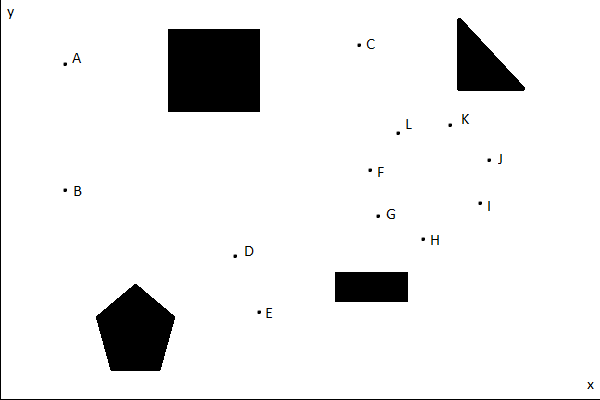
\includegraphics{drones-graphique.png}
\end{center}
\end{figure}

\end{document}
